\newpage
\section{Entwurf und Aufbau der Datensammlungsumgebung}
TBD

\subsection{Identifizierung diverser Datenströme zur Integration in einem einheitlichen Datenkorpus}
Die erste Datenquelle für die Datensammlungsumgebung ist die Anwendungsschnittstelle der Tagesschau. Diese ist eine Nachrichtensendung der Arbeitsgemeinschaft der öffentlich-rechtlichen Rundfunkanstalten der Bundesrepublik Deutschland (ARD) . Über diese Schnittstelle ist es möglich, Beiträge der Website www.tagesschau.de im JavaScript Object Notation (JSON) Format abzufragen. 
Die Schnittstelle ist mit einer OpenAPI Specification dokumentiert, über welche alle Informationen bezogen werden können. Der Zugriff auf diese Schnittstelle ist auf 60 Aufrufe pro Stunde limitiert. Darüber hinaus ist lediglich die nicht-kommerzielle Nutzung gestattet. Zudem dürfen gesammelte Inhalte, mit Ausnahme der unter der Creative Common (CC) Lizenz stehenden Inhalte, nicht weiter veröffentlicht werden. \footcite [Vgl.][]{Fischer.2024}

Die Schnittstelle gruppiert sich in 4 Themensegmente, welche über eigene Endpunkte verfügen. 
\begin{itemize}
    \item Homepage - Abfrage von Nachrichten und Eilmeldungen der Startseite
    \item News - Abfrage von sämtlichen Nachrichten und Eilmeldungen
    \item Channels - Abfrage von Kanälen
    \item Search - Allgemeine Suche über alle Inhalte der Plattform
\end{itemize}
Jeder Endpunkt ist gemäß dem Paradigma Representational State Transfer (REST) konstruiert und wird entsprechend über das Hypertext Transfer Protocol (HTTP) abgefragt. \footcite [Vgl.][]{Fischer.2024}
\newpage

Für die erste Umsetzung der Datensammlungsumgebung ist es ausreichend, den News Endpunkt zu konsumieren. Dieser gibt eine Liste von News Objekten zurück, wie im \ref{Anhang} beschrieben. Diese enthält folgende Informationen:

\begin{table}[bp!]   
    \centering
    \caption{Attribute Tageschau API Response}
    \label{tab:Attribute Tageschau API Response}
    \begin{tabular}{|c|p{11cm}|} \hline 
        news & Bildet das Hauptelement, welches die verschiedenen Nachrichten enthält \\ \hline 
        sophoraId & Eindeutige Identifikationsnummer \\ \hline 
        externalId & Zusätzliche eindeutige Identifikationsnummer \\ \hline 
        title & Titel der Nachricht \\ \hline 
        teaserImage & Enthält Informationen über das Vorschaubild der Nachricht \\ \hline 
        date & Das Veröffentlichungsdatum des Artikels \\ \hline 
        tracking & Liste von Objekten, welche Tracking-Informationen beinhalten\\ \hline 
        tags & Liste von Objekten, welche Schlagwörter enthalten \\ \hline 
        updateCheckUrl & Adresse zur Überprüfung von Aktualisierungen der Nachricht \\ \hline 
        regionId & Identifikationsnummer, welche den regionalen Bezug der Nachricht angibt \\ \hline 
        details & Adresse zum Abfragen des Artikels im JSON Format \\ \hline 
        detailsweb & Adresse zum Abfragen des Artikels im HTTP Format \\ \hline 
        shareURL & Adresse zum Artikel zum Teilen der Nachricht über soziale Medien \\ \hline 
        topline & Kurze Zusammenfassung der Nachricht \\ \hline 
        firstSentence & Erster Satz der Nachricht \\ \hline 
        geotags & Enthält eine Liste von Objekten, welche die geographischen Informationen des Artikels beinhalten \\ \hline 
        type & Typ der Nachrichtenseite, z.B. \textit{news page} \\ \hline 
        nextPage & Adresse auf die nächste Seite mit weiteren Nachrichten \\ \hline 
        comments & Adresse zur Kommentarsektion eines Artikels, sofern vorhanden \\ \hline 
        ressort & Themenfeld des Artikels, z.B. \textit{ausland} \\ \hline 
        breakingNews & Boolescher Wert, ob der Artikel als Eilmeldung veröffentlicht wurde \\ \hline
    \end{tabular}
\end{table}
\newpage
Die Informationen im Tracking Attribut werden für das Erfassen und Analysieren des Nutzerverhaltens verwendet und können entsprechend für eine Analyse sinnvoll sein. 

\begin{table}
\centering
\caption{Tracking-Objekte in der Tagesschau API}
\label{tab:Tracking Tageschau API}
\begin{tabular}{|c|p{11cm}|} \hline 
    \textbf{Tracking-Attribut} & \textbf{Beschreibung} \\ \hline 
        sid & Session Id zum Nachverfolgen des Nutzerverhaltens \\ \hline 
        src & Quelle des Artikels, zeigt z.B. auf den Kanal, aus welchem der Artikel stammt \\ \hline 
        ctp & Art des Inhaltes als technischer Kenner \\ \hline 
        pdt & Datum der Veröffentlichung (englisch: Publish Date Time) \\ \hline 
        otp & Art des Inhaltes als fachlicher Kenner, z.B. \textit{meldung} \\ \hline 
        cid & Eindeutige Identifikationsnummer \\ \hline 
        pti & Titel der Seite (englisch: Page Title) \\ \hline 
        pcr & Flaggen Attribut, Verwendung ist unbekannt \\ \hline 
        type & Typ des Tracking Objektes, z.B. \textit{generic} \\ \hline
    \end{tabular}
\end{table}
Die erste Ebene der Datenstruktur enthält primär Metadaten zu einer Nachricht. Um den, für die Sammlung relevanten, Inhalt zu erhalten, sind die Referenzen auf die Details sowie die Kommentare aufzulösen. 
Dazu wird jeweils die Adresse aus dem jeweiligen Attribut aufgerufen. 

\newpage
Die Antwort für den Artikel erfolgt als JSON Objekt. Dieses enthält ebenfalls Metadaten, wie \textit{sophoraId}, \textit{externalId}, \textit{title} und \textit{date}, darüber hinaus aber auch den Artikel selbst. 
Der Inhalt ist in verschiedene Segmente aufgeteilt und entsprechend in der JSON-Antwort abgebildet. Der Inhalt eines Segments wird im \textit{value} Attribut gehalten, im \textit{type} Attribut wird bestimmt, um was es sich handelt (text, headline, box etc.).

Die Antwort für die Kommentarsektion erfolgt als HTML Seite. 
\begin{figure}
    \centering
    
\includegraphics[width=1\linewidth]{abbildungen/Screenshot Comment Tagesschau.PNG}
    \caption{Tagesschau Kommentarsektion} 
    \label{fig:Tagesschau Kommentarsektion}
    Quelle: \fullcite{Norddeutscher_Rundfunk.2024}
\end{figure}

Aus Dieser lassen sich verschiedene Informationen beziehen.
\begin{itemize}
    \item Username
    \item Profilbild
    \item Datum und Uhrzeit des Kommentars
    \item Kommentar Text
    \item Anzahl der Antworten
    \item Anzahl der gesamten Kommentare zum Artikel
\end{itemize}

Die Kommentare werden in Seiten strukturiert und entsprechend nur teilweise zurückgegeben (engl. Paging). Dabei wird die Reihenfolge chronologisch bestimmt, beginnend mit den ersten Kommentaren. Das Konzept plant das Beziehen der ersten Seite der Kommentare.

\newpage

\begin{figure}
    \centering
    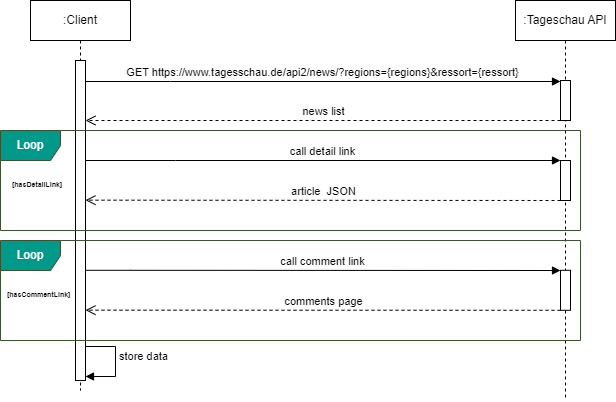
\includegraphics[width=1\linewidth]{abbildungen/Request Sequence.drawio.png}
    \caption{Abfragesequenz Datensammlung}
    \label{fig:Abfragesequenz Datensammlung}
\end{figure}
Der Ablauf der Datensammlung muss zwangsläufig mit dem initialen Abfragen der Tagesschau API starten, wie in der OpenAPI Spezifikation beschrieben. Dabei kann sowohl die Region wie auch das Ressort der gewünschten Artikel angegeben werden, um initial zu filtern. Anschließend können die Abfragen für den Artikelinhalt, sowie den Kommentaren stattfinden (siehe Abbildung \ref{fig:Abfragesequenz Datensammlung}). 
Um die Limitierung der Schnittstelle nicht zu überschreiten ist es notwendig, die zu machenden Aufrufe bestimmen zu können. Die Anzahl der benötigten Aufrufe lässt sich, auf Basis der geplanten Kommunikationsstruktur mit folgender Formel ausdrücken:

\(TotalRequests=1+(AmountArticles×2)\)

Dabei ist es möglich, die Abfragen sowohl synchron, wie auch asynchron auszuführen, um die Prozessdauer als Konsument zu reduzieren.

\newpage
\begin{figure}
    \centering
    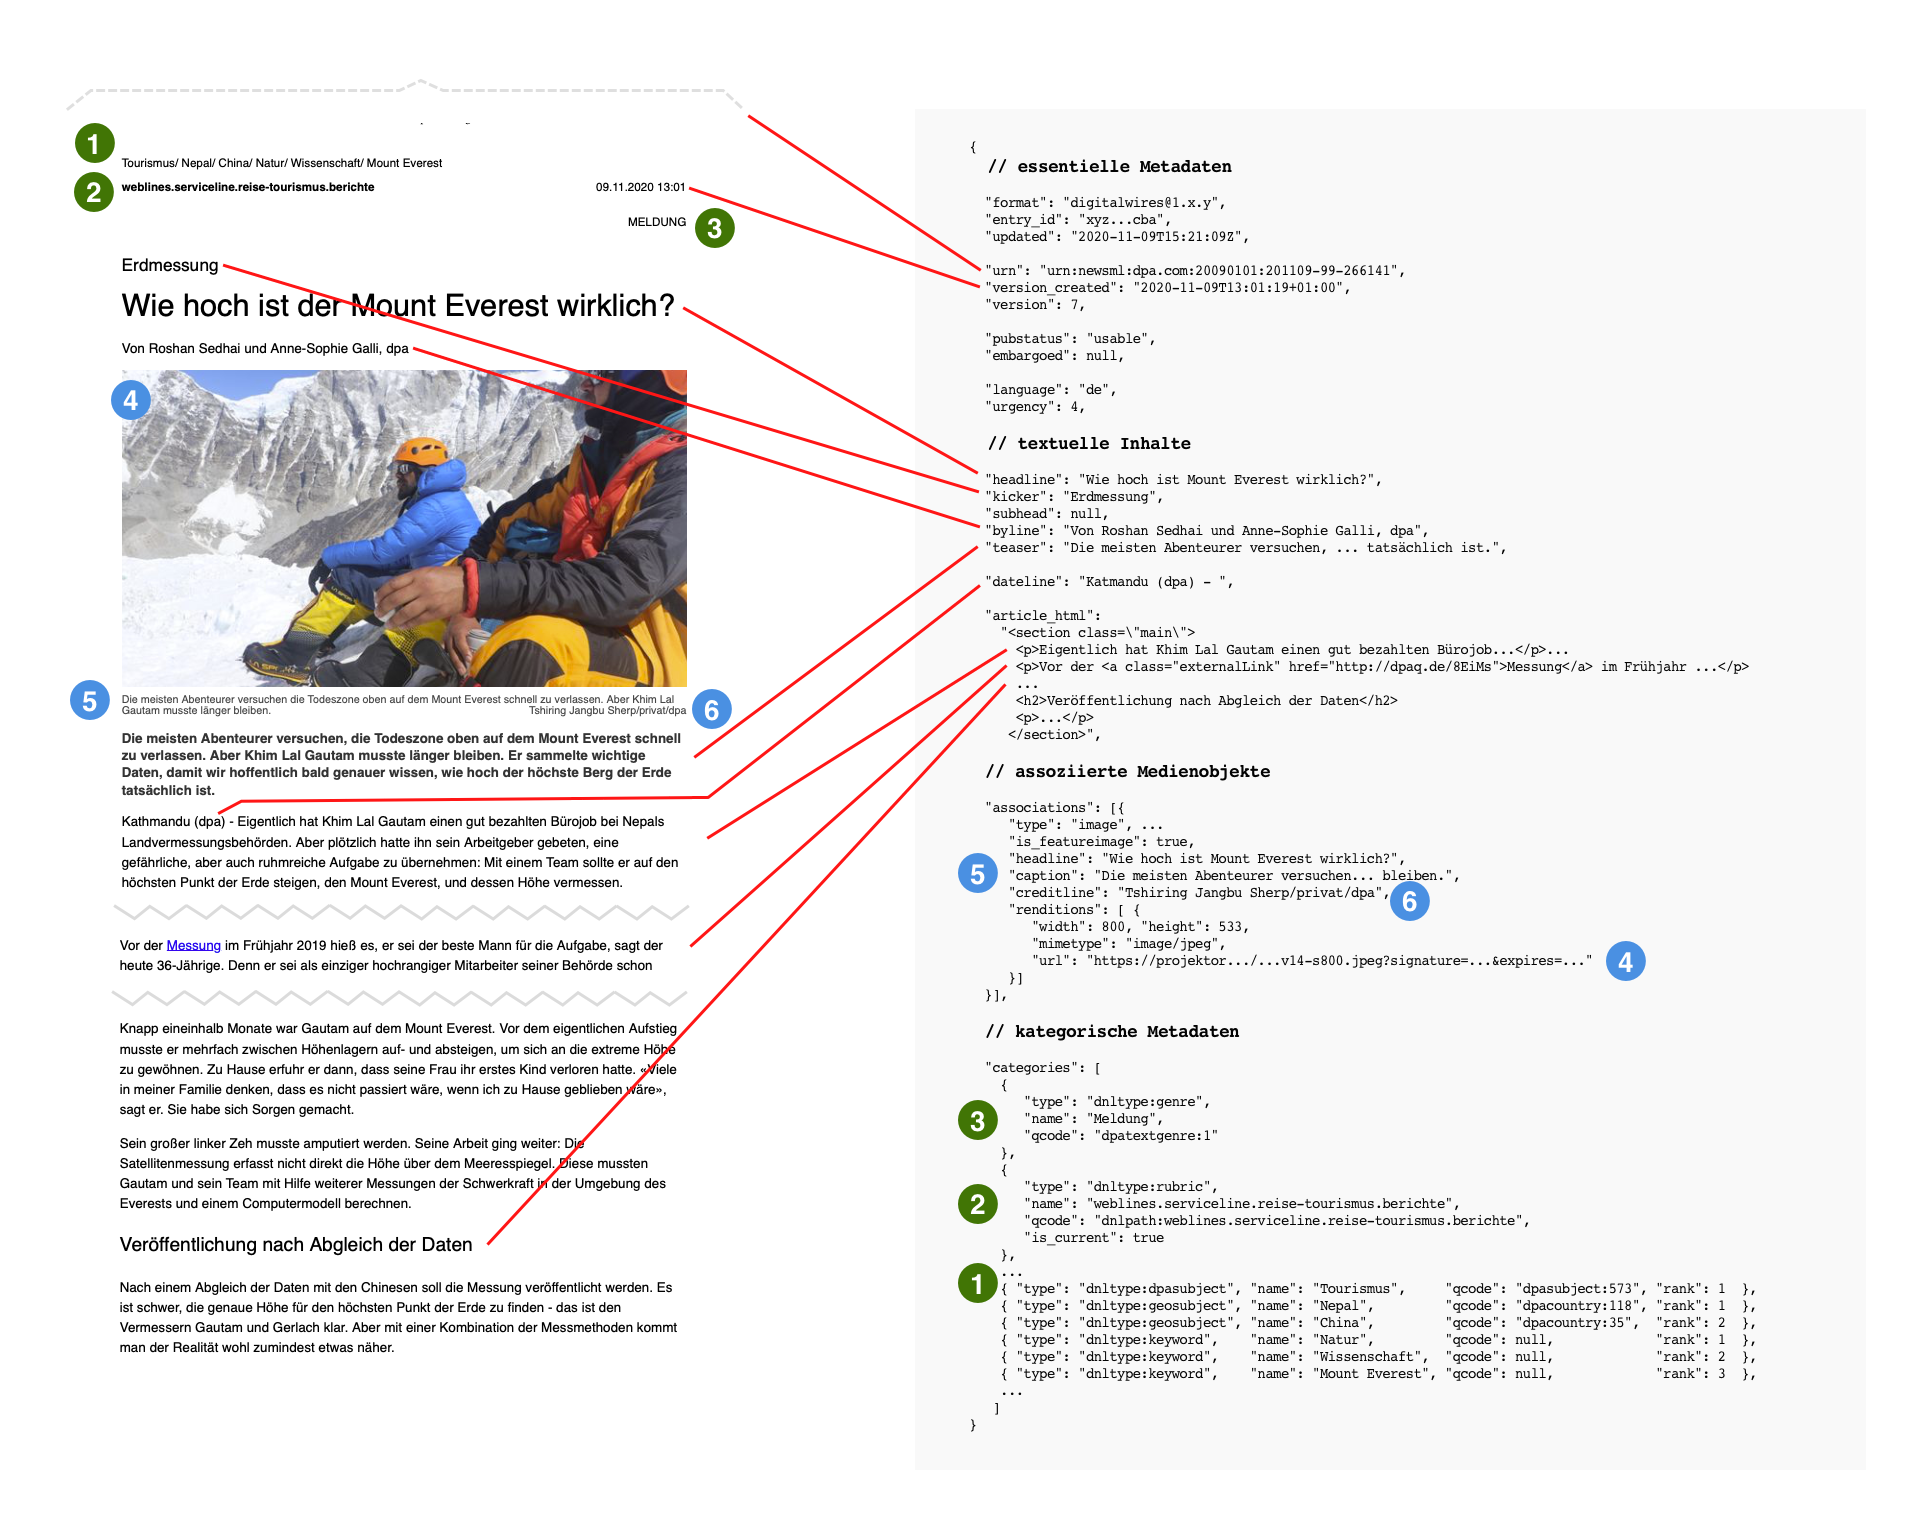
\includegraphics[width=1\linewidth]{abbildungen/dpa doc structure.png}
    \caption{Format dpa Schnittstelle}
    \label{fig:Format dpa Schnittstelle}
    Quelle: \fullcite{DpaApiDocumentation.APIs.2024}
\end{figure}
Als zweite Datenquelle wird die Deutsche Presse Agentur (dpa) angebunden. 
Diese ist die größte Nachrichtenagentur Deutschlands und möchte Inhalte möglichst neutral und unparteiisch bereitstellen.\footcite[Vgl.][]{Dpa.about.2024}

Zum maschinellen konsumieren der Nachrichten stellt die dpa mehrere APIs bereit.
Grundsätzlich werden drei Formen von Schnittstellen bereitgestellt:

\textbf{s3push-API}
Stellt die Daten im JSON Format über eine event-basierte Kommunikation bereit. Die Implementierung sieht eine direkte Anbindung eines S3 Buckets auf der Seite des Konsumenten vor und ermöglicht so das transportieren von neuen oder aktualisierten Topicles. Durch diesen Ansatz ist die Kommunikation zu der Schnittstelle wenig komplex und effizient, da als Konsument keine Logik zum aktualisieren der Bestandsdaten notwendig ist.\footcite[Vgl.][]{DpaApiDocumentation.APIs.2024}

\textbf{wireQ-API}
Stellt die Daten ebenfalls im JSON Format bereit, jedoch ausgegeben in einer cloud-basierten Warteschlange. Dadurch ist die Implementierung nicht an einem S3 Bucket gebunden, wodurch eine individuelle Kommunikationslogik auf Konsumentenseite notwendig ist. Erhalten bleibt dabei auch der Vorteil der Effizienz, da nur neue oder aktualisierte Daten transportiert werden.\footcite[Vgl.][]{DpaApiDocumentation.APIs.2024}

\textbf{jsonfeed-API}
Stellt die Daten ebenfalls im JSON Format technisch dar, welches strukturell jedoch Atom-XML bzw. RSS Feeds ähnelt. Beim Anfragen der Daten wird ein Vollbezug der verfügbaren Daten gestartet, welcher auch bereits abgefragte Nachrichten enthält. Entsprechend muss auf Konsumentenseite eine entsprechende Geschäftslogik implementiert werden. \footcite[Vgl.][]{DpaApiDocumentation.APIs.2024}
\newpage

Zu den verschiedenen Schnittstellen gibt es, bereitgestellt durch die dpa selbst, verschiedene Beispiele für Implementierungen zwecks der Anbindung an die Schnittstelle. Diese werden über Github bereitgestellt und vereinfachen, je nach Kompatibilität zu den eingesetzten Technologien, die Entwicklung des Prototypen. \footcite[Vgl.][]{dpa_newslab.github.2024}{}{}

Jede Antwort der verschiedenen Schnittstellen gliedert sich grundsätzlich in einem Container Element, welches Topicles genannt wird. Dieses organisiert die verschiedenen Nachrichteninhalte der jeweiligen Gruppen der dpa. Dadurch ergibt sich der Vorteil, verschiedene Medien wie z.B. Texte, Bilder, oder Videos in einer einheitlichen Struktur abzubilden. Zudem ist das Format darauf optimiert, maschinell verarbeitet zu werden.\footcite[Vgl.][]{DpaApiDocumentation.Format.2024}

Die Metadaten eines Topicles setzen sich aus folgenden Attributen zusammen:
\begin{table}
    \centering
    \caption{Essentielle Metadaten im Topicles}
    \label{tab:Essentielle Metadaten im Topicles}
    \begin{tabular}{|c|p{11cm}|} \hline         
        \textbf{Tracking-Attribut} & \textbf{Beschreibung} \\ \hline 
            format                  & Das Format des Entries nach Semantic Versioning.           \\ \hline
            entry\_id               & Die technische ID des Eintrages. Ein opaker Hash.          \\ \hline
            updated                 & Der Zeitstempel der Aktualisierung des Entries in UTC.     \\ \hline
            urn                     & Die URN des Hauptobjektes des Topicles.                    \\ \hline
            version\_created        & Zeitstempel der letzten Version, mit Zeitzone.             \\ \hline
            version                 & Die Version des Hauptobjektes. Ein Integer.                \\ \hline
            type                    & Der Typ des Topicles, aktuell immer composite.             \\ \hline
            pubstatus               & Status der Veröffentlichung, z.B. "usable", "withheld".    \\ \hline
            signal                  & Hinweise zum Anlass der Veröffentlichung.                  \\ \hline
            embargoed               & Zeitstempel einer Sperrfrist, mit Zeitzone.                \\ \hline
            language                & Die Sprache des Topicles.                                  \\ \hline
            urgency                 & Die Dringlichkeit der Meldung, Integer zwischen 1 und 9.   \\ \hline
    \end{tabular}

    Quelle: Vgl. \fullcite{DpaApiDocumentation.Format.2024}
\end{table}

Darüber hinaus weisen die individuellen Datentypen unterschiedliche Attribute auf. Für die erste Iteration der Datensammlungsumgebung sind zunächst die Nachrichtentexte von Relevanz. 
Die Nachrichtentexte der Topicles weisen folgende spezielle Attribute auf:

\begin{table}
    \centering 
    \caption{Nachrichtentext im Topicles}
    \label{tab:Nachrichtentext im Topicles}
    \begin{tabular}{|c|p{11cm}|} \hline    
    \textbf{Tracking-Attribut} & \textbf{Beschreibung} \\ \hline 
        kicker                  & Die Dachzeile des Artikels.                                 \\ \hline
        headline                & Die Hauptüberschrift des Artikels.                         \\ \hline
        subhead                 & Die Unterzeile des Artikels.                              \\ \hline
        teaser                  & Der Teaser des Artikels.                                  \\ \hline
        byline                  & Die Autorenzeile des Artikels.                            \\ \hline
        dateline                & Die Ortszeile des Artikels.                               \\ \hline
        article\_html           & Der eigentliche Artikeltext als HTML <section>.            \\ \hline
        infobox\_html           & Die zum Artikel gehörende Infobox als HTML <section>.      \\ \hline
        linkbox\_html           & Externe Links als HTML <section>.                          \\ \hline
        creditline              & Die Agenturzeile / Urheberzeile des Artikels.             \\ \hline
        copyrightnotice         & Der Copyright-Hinweis für den Artikel.                    \\ \hline
        usageterms              & Die urheberrechtlichen Nutzungsbedingungen.                \\ \hline
        autopublishnotice       & Der Urheberrechtshinweis für automatisierte Publikationen. \\ \hline
        ednotes                 & Redaktionelle Hinweise zum Artikel. Liste von Objekten.    \\ \hline
        descriptions            & Liste von Beschreibungen. Verschiedene Texte im Key description. \\ \hline
    \end{tabular}

    Quelle:  Vgl. \fullcite{DpaApiDocumentation.Format.2024}
\end{table}

\newpage
\subsection{Bildung eines Datenkorpus für eine Sentiment Analyse}
Die Struktur des, zur Analyse benötigten, Datenkorpus bildet sich aus den Schlüsselelementen der beiden Dokumentenkorpora. Dabei sind Attribute relevant, welche in der Schnittmenge der beiden Strukturen liegen, sind jedoch nicht darauf beschränkt. 
\begin{table}
    \centering
\caption{Struktur Datenkorpus für Nachrichtenartikel}
\label{tab:Datenkorpus}
    \begin{tabular}{|c|c|c|c|}
         Name Datenkorpus&  Attribut Tagesschau&  Attribut dpa& Beschreibung \\
         id&  sophora_id&  entry_id& Eindeutiger Identifier für einen Artikel \\
         title&  title&  headline& Überschrift des Artikels \\
         date&  date&  version_created& Zeitstempel Erstellung des Artikels \\
         teaser&  firstSentence&  teaser& Kurze Einführung in den Artikel \\
         language&  (Annahme: deutsch)&  language& Sprache des Artikels \\
         usageterms&  (Annahme: Spezifische Nutzungsbedingungen)&  usageterms& Nutzungsbedingungen der Inhalte \\
         text_content&  details&  article_html&  Inhalt des Artikels\\
        comments& (Konstruiert aus Abfrage)& (nicht gegeben)&Besteht aus: 
        Username
        Datum und Uhrzeit des Kommentars
        Kommentar Text\\
    \end{tabular}
    
    
\end{table}
Neben den relevanten Attributen aus der Schnittmenge, wurde auch \textit{language}, \textit{usageterms} sowie \textit{comments} eingeführt. Im aktuellen Szenarion können die nicht explizit gepflegten Werte aus der Tagesschau durch den Kontext heraus gefüllt werden, da sowohl die Sprache, als auch die Nutzungsbedienungen fest definiert werden können. Die Kommentare sind bei der dpa gar nicht vorhanden, jedoch bei der Tagesschau auch nicht pauschal verfügbar. Das Einführen des Attributs in den Korpus ermöglicht jedoch das Abbilden solcher Inhalte, insbesondere im Hinblick auf die Erweiterbarkeit.

Die Struktur des Datenkorpus ermöglicht auch weitere, bisher unbekannte, Datenquellen einzubinden. Seine Struktur ist allgemeingültig für Nachrichtenartikel, da er auf die essenziellen Informationen reduziert ist. 
Dadurch wird die Erweiterbarkeit weiter verbessert.

\newpage
\subsection{Architektur und Design der Datensammlungsumgebung}
Zur Erarbeitung der Architektur ist es notwendig, die gegeben Rahmenbedingungen (engl. constraints) zu definieren und daraus nicht- funktionale Anforderungen zu definieren. Daraus ist herauszustellen, welche Qualitätsmerkmale das System verfolgt. 

Als  Randbedingungen für die Datensammlungsumgebungen gelten alle Einschränkungen der genutzten Schnittstellen. Diese weisen unterschiedliche Nutzungsbedienungen auf, welche in der Architektur berücksichtigt und eingehalten werden müssen. Darüber hinaus ist zu beachten, wie die Daten vorgehalten werden um ebenfalls , im Bezug auf Privatsphäre, konform zu arbeiten. 

Das detaillierte Dokumentieren der Architektur verbessert die Transparenz über den Datenbezug, sowie der Datenverarbeitung. Dieser Aspekt ist essentiell wichtig, um den Anspruch der Nachvollziehbarkeit gerecht zu werden, da sich daraus auch ggf. vorliegende Limitierungen in der Erhebung bzw. Analyse nachvollziehen lassen.\footcite[Vgl.][]{Sayogo.Challenges.2015}{}{}

[Erweitern um ethische Aspekte ggf.]

Für die Datensammlungsumgebung ist die Datenqualität das wichtigste Merkmal. Es entscheidet darüber, wie erfolgreich die nach-gelagerten Analysen ausfallen werden, welche die Begründung für diese Umgebung darstellen. Datenqualität umfasst unter anderem die Aspkete Genauigkeit, Gültigkeit, Vollständigkeit und Verfügbarkeit.
Durch einen erhöhten Anspruch an die Datenqualität wird das Datenvolumen reduziert, da mehr Informationen gespeichert werden. Zum Evaluieren der Datenqualität kann initial eine explorative Analyse auf Basis der extrahierten Daten vorgenommen werden. Im produktiven Betrieb der Umgebung kann die Qualität der Analyseergebnisse betrachtet werden. \footcite[Vgl.][]{Kilkenny.Data.2018}

Als weiteren Aspekt der Umgebung steht die Erweiterbarkeit bzw. die Flexibilität im Fokus. Der fachliche Anspruch ist es, verschiedene Datenströme zu integrieren. Durch das Einbinden verschiedener Datenquellen können mehr Daten gesammelt werden. Im Kontext der Berichterstattung werden dadurch auch verschiedene Perspektiven auf die selben Themen abgebildet, was weitere Analysemöglichkeiten eröffnet. Das extrahieren der Texte aus den Nachrichtenartikeln muss so konstruiert sein, dass  bei Änderungen am Format der Texte, die Schnittstelle entsprechend funktional bleibt bzw. möglichst schnell angepasst werden kann. Wie flexibel die Architektur im Bezug auf sich ändernde Anforderungen reagiert, lässt sich ansatzweise über die benötigte Zeit zur Bereitstellung einer Anpassung (engl. Time to Market) bestimmen, bzw. bei weitreichenderen Bedarfen über eine graphenbasierte Representation der Anwendung.\footcite[Vgl.][]{Broniatowski.Measuring.2016}{}{}

Für die erste Iteration der Anwendung ist die Wartbarkeit, sowie die Benutzerfreundlichkeit zu vernachlässigen, da diese sich konkurrierend zu der Idee eines Prototypen verhalten. Dadurch wird eine schnelle Entwicklung zu Beginn ermöglicht, wodurch der erste vollständige Prozess der Datenverarbeitung frühzeitig durchlaufen werden kann. Daraus resultieren frühzeitig Erkenntnisse, welche für die Qualität der Datensammlungsumgebung essentiell sind.\footcite[Vgl.][]{Strang.Mining.2023}{}{}

[Inhalt zur angestrebten Analyse]

\textbf{Komponenten der Systemarchitektur}
Der erster Prozess-schritt der Datensammlungsumgebung ist das Abfragen der verschiedenen Nachrichten-Quellen. Die Komponente muss dazu in der Lage sein, entsprechende HTTP Aufrufe an die die Schnittstellen der Nachrichtenquellen zu richten. Dabei ist die Restriktion der Aufrufe bei der Tagesschau zu beachten. Im Bereich von öffentlichen Schnittstellen sei es nach Fresno-Aranda zu erwarten, dass diese Einschränkung bei weiteren Schnittstellen ebenfalls auftreten werden.\footcite[Vgl.][]{Fresno-Aranda.Automated.2022}{}{}

Diese Aufgabe wird durch einen  bzw. mehrere  Microservices erfüllt, welche es ermöglichen, die jeweilgen Schnittstellen abzufragen.  So kann, je nach Bedarf, die Logik zur Abfrage der Nachrichtenartikel auf die Services aufgeteilt werden, sodass je angebundener Quelle ein Microservice das Abfragen sowie das temporäre Speichern der Dokumentenkorpora vornehmen kann. 

Die verschiedenen Services können unabhängig voneinander entwickelt werden, wodurch jeweils die passende Technologie, wie z.B. Programmiersprachen, Frameworks etc. , verwendet werden können. 

Zudem sind Diese getrennt skalierbar, um kosteneffizent die unterschiedlichen Bedarfe an die Ressourcen des Systems zu adressieren. Dies ist insbesondere für die Schnittstelle der dpa interessant, da diese eine native Unterstützung zur Speicherung in einen S3 Bucket ermöglicht. 

Als Datenbanksystem eignet sich die Technologie MongoDB, welche das Speichern von Dokumentenkorpora ermöglicht, bevor diese strukturiert wurden. Dadurch können Rohdaten temporär vorgehalten werden, um die Verarbeitung der Rohdaten als Stapelverarbeitung anstelle einer Echtzeitverarbeitung zu gestalten. Dadurch kann die Datensammlungsumgebung die Aufwände effizient verteilen. 
Zudem reduziert das die Komplexität von Fehlerbehebung, da der Datenfluss nicht unmittelbar unterbrochen wird.

Der zu entwickelnde Prototyp muss entsprechend das Abfragen der Schnittstellen vornehmen und das Ablegen in eine Datenbank abbilden. 
Der Prototyp speichert die Resultate, der verschiedenen Datenquellen, in einen zentralen Speicher beispielsweise im Dateisystem des Entwicklungsrechner. 
Bei der angestrebten Weiterentwicklung auf die Microservice Architektur würde eine Datenbank je Microservice implementiert werden. Dadurch wird das Konzept der losen Kopplung zwischen den Services bewahrt auf Kosten der Komplexität, sowie den Betriebskosten. Dies würde die Funktionen eines Data Lakes abbilden, dabei jedoch selektiv skalierbar sein. \footcite[Vgl.][]{Iatropoulou.BigDataServices.2021}{}{}

Die Architektur gliedert sich in verschiedenen Schichten (engl. Layered Architecture) um eine entsprechende Struktur zu etablieren und den Fokus auf die lose Kopplung zu forcieren. Das klare Abgrenzen in die verschiedenen Schichten erlaubt zudem die Abstraktion der Komplexität, welche durch die gewählte Architektur entsprechend amplifiziert ist. Zudem wirkt sich diese Strukturierung förderlich auf die Wiederverwendbarkeit sowie die Performance des Systems aus.\footcite[Vgl.][]{Wang.LayeredMicroservices.2018}{}{}

Die, zur Abfrage der Nachrichtenseiten konzipierten, Microservices inklusive deren Datenbanken bilden die \textit{Storage Layer.} Die Nachrichtenseiten gliedern sich in der abstrakten Schicht External Sources.

Die Kommunikation der Microservice untereinander wird durch einen zentralen Dienst (engl. Event Streaming Plattform) gesteuert, welcher Ereignisse (engl. Events) durch die Microservices enthält und bereitstellt. Auf diese können andere Microservices reagieren und definierte Verarbeitungen durchführen. Beispielsweise kann ein Microservice aus dem \textit{Storage Layer} ein Ereigniss an den Event Broker senden, sobald ein neuer Artikel bezogen wurde. Dies stärkt die Entkopplung, sowie die Erweiterbarkeit, als auch die Skalierbarkeit der finalen Architektur auf Kosten der Komplexität des Systems.
Mögliche Technologie zur Realisierung der Event Streaming Plattform wäre Kafka der Firma Apache.\footcite[Vgl.][]{Kul.PublishSubscribeMicroservices.2021}{}{}

Im nächsten Schritt müssen die Daten für die Analyse prozessiert werden. Dazu wird ein weiterer Microservice implementiert, welcher zudem einem entsprechendem Datenspeicher zugeordnet ist, beispielsweise einem Serverless Data Warehouse oder einem Cloud Storage. 
Dieser Service greift auf die Daten der Services der \textit{Storage Layer} zu und prozessiert diese gemäß den Anforderungen der nach-gelagerten Analyseschritte. 
Die Microservices konsumieren die Events aus der Event Streaming Plattform und starten daraufhin ihre Prozessierung.

Durch diese Form der Gestaltung ist es möglich, mehrere verschiedene Prozessierungen für verschiedene Analysen bereitzustellen, durch das Implementieren weiterer Microservices. Zudem entsteht durch die Kapselung der Prozessierung eine Virtualisierung der vorgehaltenen Daten, welche den Zugriff auf die Daten, durch Konsumenten, verbessert. Diese Komponenten gliedern sich in dem \textit{Processing Layer}.

Im letzten Prozess-schritt werden die prozessierten Daten abgefragt und durch entsprechende Analysen verwendet. Dies wird durch entsprechende Analytics Microservices abgebildet, welche sich je nach gewünschter Struktur der Analyse, aufbauen lassen. Diese Services konsumieren die Events der \textit{Processing Layer} und starten daraufhin ihre Verarbeitung. Durch den modularen Aufbau der Architektur, sowie dem vorhalten der Dokumenten- und Datenkorpora ist es möglich, dies Analyse last-gerecht nach dem Prinzip der Stapelverarbeitung durchzuführen.
Zudem können, je nach Analyse, utnerschiedliche Technologien in die Architektur integriert werden.
Sollte ein Anwendungsfall (engl. Use Case) eine Analyse mit Echtzeitverarbeitung benötigen, kann die gegebene Architektur dies ebenfalls abbilden.\footcite[Vgl.][]{Hsu.MicroserviceAnalyticsPlattform.2018}{}{}

Die geplanten Komponenten lassen sich in folgender Systemlandschaft abbilden.

\begin{figure}
    \centering
    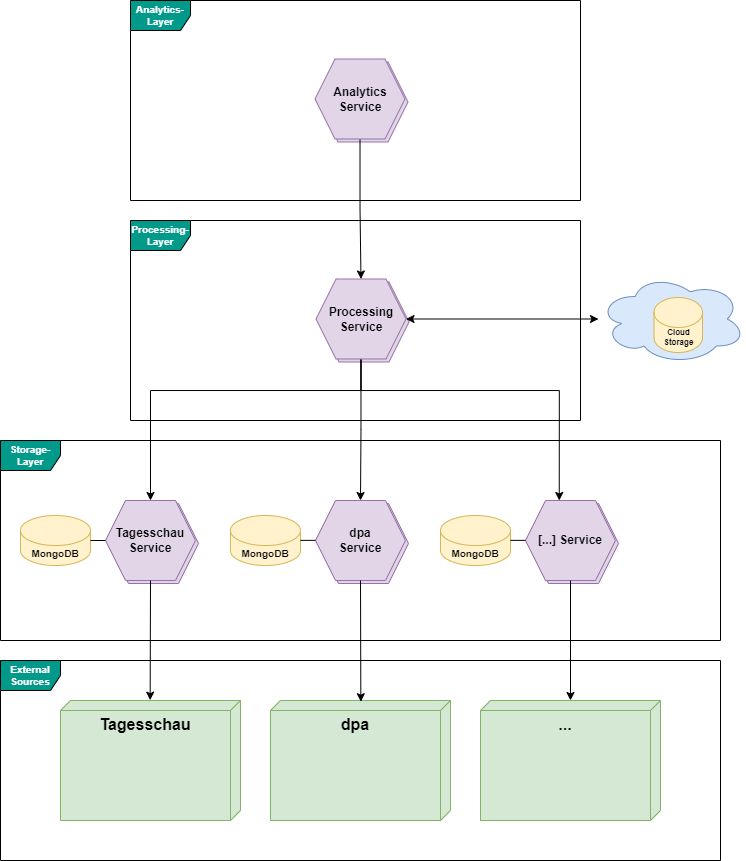
\includegraphics[width=0.5\linewidth]{abbildungen/System Architektur.drawio.png}
    \caption{System Architektur Modell}
    \label{fig:system-architecture}
\end{figure}
\newpage
Um die technische Machbarkeit der geplanten Architektur, zu evaluieren, werden die Kernfunktionalitäten der Architektur abgebildet. Diese beinhalten das Abfragen der Nachrichtenseiten, das prozessieren dieser Daten als Vorbereitung auf die Analyse, sowie die Analyse selbst. 
Als technische Basis eignet sich eine Implementierung als Jupiter Notebook, da sich auf dieser Basis diese Funktionen ohne große Komplexität abbilden lassen. 
Die Stapelverarbeitung wird dabei als Batch Job lokal programmiert, um die Limitierung der Tagesschau einzuhalten. Zudem kann die Analyse ebenfalls im Notebook abgebildet werden. 
Die daraus generierten Erfahrungen können bei der Implementierung der Systemarchitektur dann berücksichtigt werden, bevor getroffene Entscheidungen endgültig werden.

\begin{figure}
    \centering
    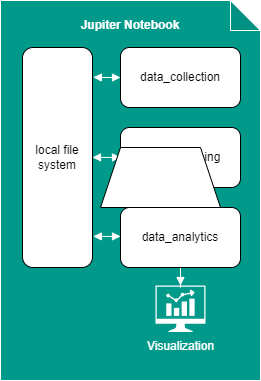
\includegraphics[width=0.5\linewidth]{abbildungen/Prototyp Architecture.drawio.png}
    \caption{Prototyp Software Architektur}
    \label{fig:prototyp-architecture}
\end{figure}